\documentclass[tikz,border=5pt]{standalone}
\usepackage{tikz}
\usetikzlibrary{shapes, arrows, positioning, calc}

\begin{document}
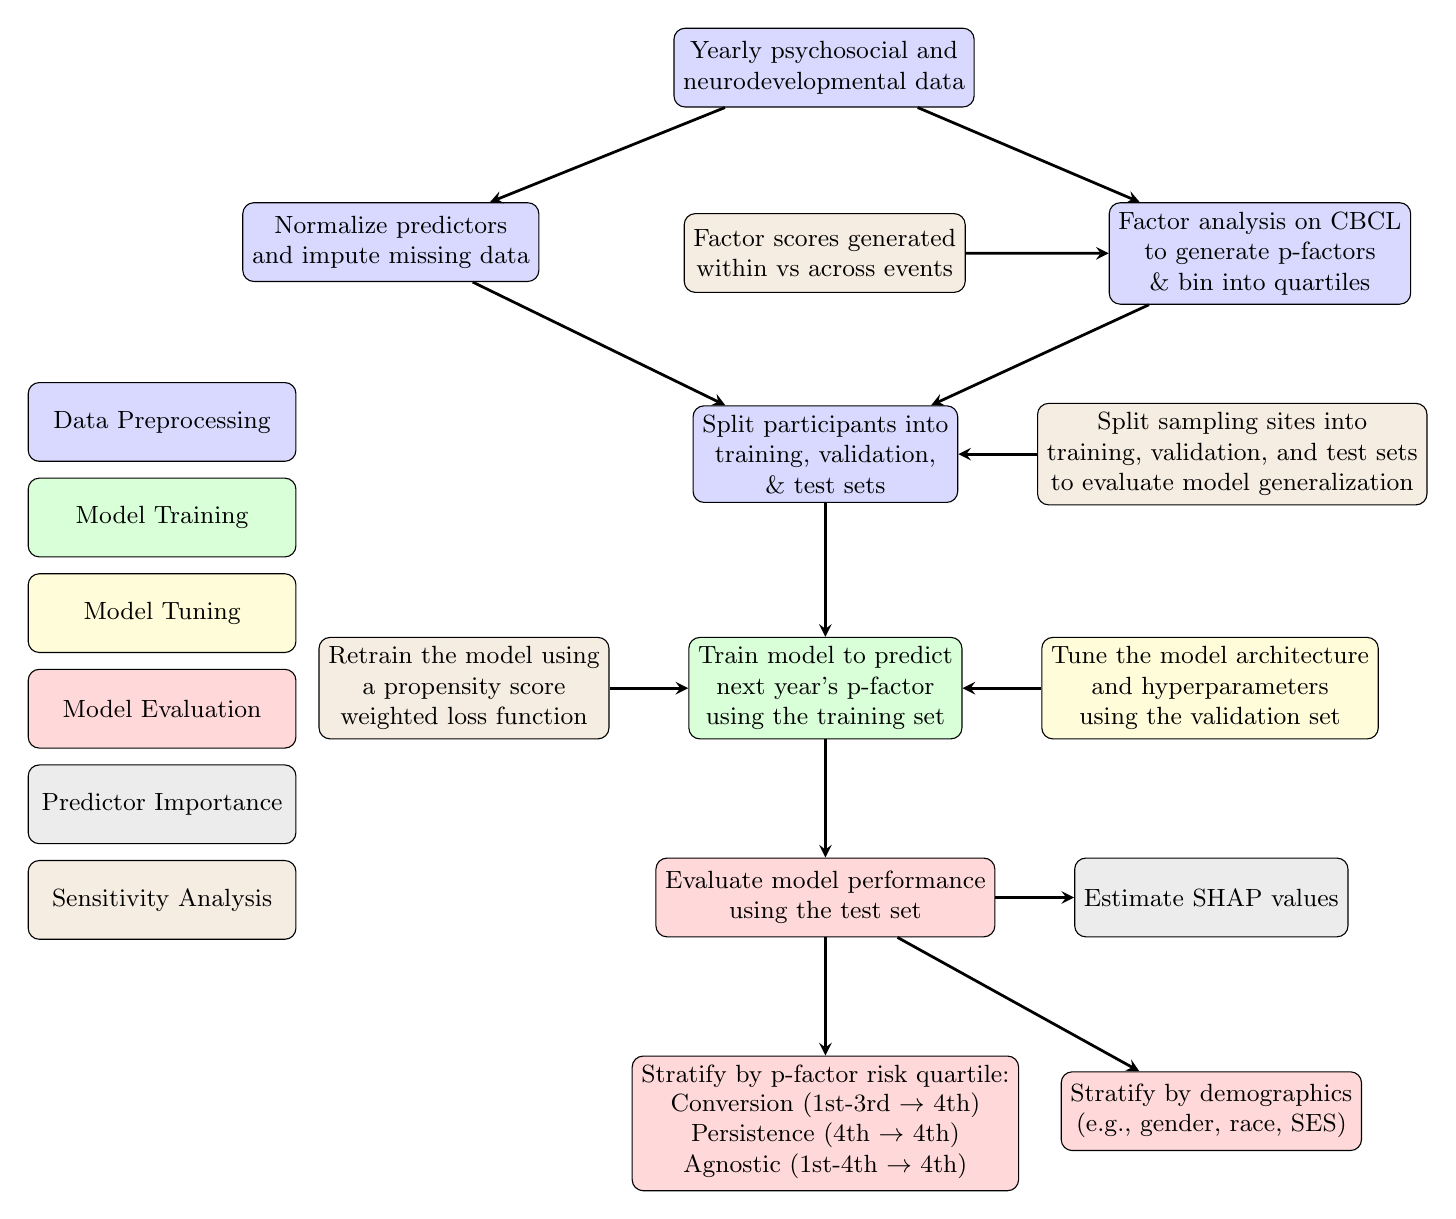
\begin{tikzpicture}[node distance=1.7cm,
    every node/.style={font=\small}, 
    >=latex, 
    box/.style={rectangle, draw=black, rounded corners, align=center, minimum width=2.5cm, minimum height=1cm}, 
    line/.style={draw, -stealth, line width=1pt}]

% Data Preprocessing
\node[box, fill=blue!15] (data) at (0,0) {Yearly psychosocial and\\neurodevelopmental data};
\node[box, fill=blue!15, below left=of data, xshift=-0.5cm] (prep) {Normalize predictors\\and impute missing data};
\node[box, fill=blue!15, below right=of data, xshift=0.5cm] (factor) {Factor analysis on CBCL\\to generate p-factors\\\& bin into quartiles};
\node[box, fill=blue!15, below=2cm of $(prep)!0.5!(factor)$] (split) {Split participants into\\training, validation,\\\& test sets};

% Model Training
\node[box, fill=green!15, below=of split] (train) {Train model to predict\\next year's p-factor\\using the training set};

% Model Evaluation + Predictor Importance
\node[box, fill=red!15, below=1.5cm of train] (test) {Evaluate model performance\\ using the test set};
\node[box, fill=gray!15, right=1.0cm of test] (shap) {Estimate SHAP values};
\node[box, fill=red!15, below=1.5cm of test] (stratify) {Stratify by p-factor risk quartile:\\\begin{tabular}{c}Conversion (1st-3rd $\to$ 4th)\\Persistence (4th $\to$ 4th)\\Agnostic (1st-4th $\to$ 4th)\end{tabular}};
\node[box, fill=red!15, right=of stratify, below=of shap] (demo) {Stratify by demographics\\(e.g., gender, race, SES)};

% Sensitivity Analysis
\node[box, fill=brown!15, right=1.0cm of split] (site) {Split sampling sites into\\training, validation, and test sets\\to evaluate model generalization};
\node[box, fill=brown!15, left=1.0cm of train] (propensity) {Retrain the model using\\a propensity score\\weighted loss function};
\node[box, fill=brown!15, yshift=0.1cm] (factormodel) at ($(data)!0.5!(split)$) {Factor scores generated\\ within vs across events};

% Model Tuning
\node[box, fill=yellow!15, right=1.0cm of train] (tune) {Tune the model architecture\\and hyperparameters\\using the validation set};

% Legend
\node[box, fill=blue!15, left=of split, minimum width=3.4cm, yshift=0.5cm] (legend1) at (-5,-5) {Data Preprocessing};
\node[box, fill=green!15, below=0.2cm of legend1, minimum width=3.4cm] (legend2) {Model Training};
\node[box, fill=yellow!15, below=0.2cm of legend2, minimum width=3.4cm] (legend3) {Model Tuning};
\node[box, fill=red!15, below=0.2cm of legend3, minimum width=3.4cm] (legend4) {Model Evaluation};
\node[box, fill=gray!15, below=0.2cm of legend4, minimum width=3.4cm] (legend5) {Predictor Importance};
\node[box, fill=brown!15, below=0.2cm of legend5, minimum width=3.4cm] (legend6) {Sensitivity Analysis};

% Paths
\draw [line] (data) -- (prep);
\draw [line] (data) -- (factor);
\draw [line] (prep) -- (split);
\draw [line] (factor) -- (split);
\draw [line] (split) -- (train);
\draw [line] (tune) -- (train);
\draw [line] (train) -- (test);
\draw [line] (test) -- (stratify);
\draw [line] (test) -- (demo);
\draw [line] (factormodel) -- (factor);
\draw [line] (test) -- (shap);
\draw [line] (site) -- (split);
\draw [line] (propensity) -- (train);

\end{tikzpicture}
\end{document}
